\documentclass[
	12pt,
	a4paper,
	draft
]{report}

\usepackage[english,ngerman]{babel}
\addto{\captionsngerman}{\renewcommand{\abstractname}{Abstract}}
\usepackage[utf8]{inputenc}
\usepackage[a4paper, left=3.5cm, right=2.5cm, top=2.5cm, bottom=2cm]{geometry}
\usepackage[nottoc]{tocbibind}

\usepackage[
	colorlinks=true,
	citecolor=blue,
	linkcolor=black,
	filecolor=black,
	urlcolor=blue,
	linktoc=all
]{hyperref}

\usepackage{graphicx}
\graphicspath{ {img/} }
\usepackage{subcaption}

\usepackage[babel]{csquotes}
\MakeOuterQuote{"}

\usepackage[
	backend=biber,
	style=trad-abbrv,
	minbibnames=10,
	maxbibnames=10,
	maxcitenames=2,
	giveninits=true,
	eprint=false,
]{biblatex}
\AtEveryBibitem{
	\clearlist{language}
	\clearfield{note}
	\clearfield{eventtitle}
	\clearfield{booksubtitle}
	\ifentrytype{misc}{
	}{
	\clearfield{url}
	}
}
\addbibresource{references.bib}
\DefineBibliographyStrings{german}{
	andothers = {et\addabbrvspace al\adddot},
	andmore = {et\addabbrvspace al\adddot},
}

% Erklärung
\usepackage{multicol}

% Acronyms
\usepackage[acronym]{glossaries}
\glstoctrue
\makeglossaries

\newacronym{cnn}{CNN}{Convolutional Neural Network}
\newacronym{rnn}{RNN}{Recurrent Neural Network}
\newacronym{wce}{WCE}{Wireless Capsule Endoscopy}
\newacronym{nbi}{NBI}{Narrow-Band Imaging}
\newacronym[plural=NN,firstplural=Neuronale Netze (NN)]{nn}{NN}{Neuronales Netz}
\newacronym{svm}{SVM}{Support Vector Machine}
\newacronym{fc}{FC}{Fully Connected}
\newacronym{fcn}{FCN}{Fully Convolutional Network}
\newacronym{gan}{GAN}{Generative Adversarial Network}
\newacronym{dcgan}{DCGAN}{Deep Convolutional GAN}
\newacronym{can}{CAN}{Conditional Adversarial Network}
\newacronym{gi}{GI}{Gastrointestinaltrakt}

\makeindex


\title{Segmentierung von Polypen in Koloskopie-Bilddaten mit Conditional Adversarial Networks}
\author{Josia Scheytt}

\begin{document}

\thispagestyle{empty}
\titleGM
\clearpage


\pagenumbering{roman}

\tableofcontents

\clearpage
\addcontentsline{toc}{chapter}{\abstractname~(Deutsch)}
\begin{abstract}
	Kolorektale Karzinome haben eine hohe Sterblichkeitsrate, wenn sie spät entdeckt werden.
Eine frühzeitige Entfernung von bösartigen Polypen im Magen-Darm-Trakt, die deren Vorstufen bilden, bietet jedoch hohe Überlebenschancen.
Bei Darmspiegelungen werden gerade kleine Polypen häufig übersehen.
Bildverarbeitende Systeme, die Polypen in einem Koloskopie-Frame nicht nur detektieren, sondern auch pixelgenau segmentieren, könnten Ärzten bei Darmkrebs-Screenings helfen.

Diese Masterarbeit setzt zum ersten Mal ein \acrlong{can} zur binären Segmentierung von Kolorektalpolypen ein.
Die optimale Batch-Größe sowie verschiedene Augmentierungstechniken werden evaluiert hinsichtlich der Stabilisierung des Trainings und einer Verbesserung der Ergebnisse.
Durch die Deaktivierung von Dropout zur Inferenzzeit und eine Batch-Größe von 32 werden Intersection-over-Union-Werte von bis zu 0,3681 erzielt.

\end{abstract}

\clearpage
\addcontentsline{toc}{chapter}{\abstractname~(Englisch)}
\begin{otherlanguage}{english}
\begin{abstract}
	Colorectal cancer has a high death rate when detected in a late stadium.
Early removal of their precursors -- malignant polyps in the gastrointestinal tract -- exhibits high survival rates.
During colonoscopy small polyps are easily missed.
Image processing systems that not only detect the presence of polyps but also segment them with pixel accuracy could aid doctors in colon screenings.

This master's thesis employs \acrlongpl{can} for the first time in the context of binary segmentation of colorectal polyps.
Best batch size and several dataset augmentation schemes are evaluated regarding training stabilization and improving results.
By deactivating dropout at inference time and using a batch size of 32 Intersection over Union values of up to 0.311 are reached.

\end{abstract}
\end{otherlanguage}

\pagenumbering{arabic}

\chapter{Wissenschaftliche Vertiefung}

\section{Einführung}

Unter den 20 häufigsten Todesursachen weltweit kommen auch 4 Krebsarten vor~\cite{Lozano.2012}.
Von allen Krebsarten kommen Darmkarzinome am dritthäufigsten vor, und sie sind die Krebsart mit der vierthöchsten Sterblichkeitsrate~\cite{Ferlay.2012}.
Kolorektale Karzinome, also Krebs im Blinddarm oder Dickdarm, machen davon den allergrößten Anteil aus~\cite{Kumar.2005}.
Wenn bösartige kolorektale Polypen frühzeitig entfernt werden, lässt sich die Mortalität verringern~\cite{Zauber.2012}.
Ein Entfernen sämtlicher Polypen inkl. der gutartigen hingegen birgt Risiken wie Blutungen und Perforation des Darmes~\cite{Rex.2009}.

Zur genaueren Untersuchung des Dickdarms und der letzten Zentimeter des Dünndarms wird oft eine Darmspiegelung (Koloskopie) durchgeführt~\cite{Schachschal.2010}.
Dieses nichtinvasive Verfahren ermöglicht eine detaillierte visuelle Inspektion des Dickdarms über ein rektal eingeführtes Koloskop.
Findet der Arzt Polypen (wie z.~B. in \autoref{fig:polyp}), kann von dem verdächtigen Gewebe direkt eine Probe entnommen werden.
Eine solche Biopsie kann dann histologisch auf Gut- oder Bösartigkeit untersucht werden.

\begin{figure}[h]
	\centering
	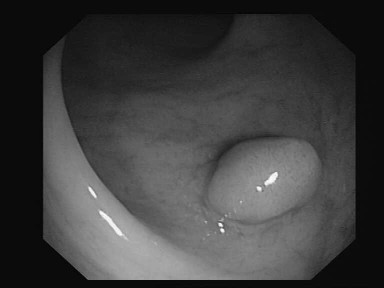
\includegraphics[width=.45\textwidth]{polyp129}

	\vspace{\baselineskip}

	
\includegraphics[width=.45\textwidth]{segm129}
	\caption{Polyp im Dickdarm (oben), Segmentierung des Polypen (unten)}
	\label{fig:polyp}
\end{figure}



\section{Problemstellung und Motivation}

Viele kleinere Polypen, die sich später zu Karzinomen entwickeln können, sind aufgrund ihrer Größe bei Koloskopien nicht einfach zu erkennen.
Mithilfe von Algorithmen, die automatisiert Polypen in Videomaterial von Koloskopien auffinden, könnte man die Arbeit des Arztes erleichtern und den Anteil an gefundenen Polypen erhöhen.
Solche Systeme könnten potenziell auch weiterentwickelt werden, sodass sie eine Abschätzung bezüglich der Gut- oder Bösartigkeit des Gewebes durchführen.

Ebenso wäre wahrscheinlich auch ein Einsatz bei einer Spiegelung des Dünndarms möglich.
Karzinome im Dünndarm kommen zwar deutlich seltener vor als im Dickdarm~\cite{Kumar.2005}, aber auch dort stellen Polypen ein Krebsrisiko dar.
Bei Dünndarm-Spiegelungen kommen häufig Endoskopkapseln zum Einsatz (\gls{wce}), wobei eine große Menge an Videomaterial anfällt, das nachträglich vom Arzt untersucht werden muss und durch Automatisierung schneller bewertbar wäre.

In dieser Arbeit werden bisherige Forschungsarbeiten vorgestellt und verglichen, die sich mit der Segmentierung von Polypen in Koloskopie-Bilddaten beschäftigen.
Dazu wird in \autoref{sec:manuelle-feature-selection} auf Methoden eingegangen, bei denen die Features für die Segmentierung manuell gewählt wurden.
Darüber hinausgehend wird in \autoref{sec:deep-learning} untersucht, inwiefern Methoden aus dem Bereich Deep Learning in diesem Anwendungsfeld einen Vorteil bieten.

Arbeiten, die nur die \emph{Präsenz} von Polypen detektieren werden hier nicht behandelt.
Im Fokus stehen Ansätze, die pixelgenaue Segmentierungen (s.~\autoref{fig:polyp}) produzieren, weil nur dadurch eine präzise Lokalisierung von Polypen im Bild möglich ist.



\section{Manuelle Feature Selection}\label{sec:manuelle-feature-selection}

In den folgenden Abschnitten wird aufgezeigt, welche Techniken bisher schon verwendet wurden, um Polypen zu segmentieren.
Einige dieser Ansätze arbeiten auch auf Bildmaterial von Untersuchungen mit \gls{wce}.

Da es sich hier um eine Problemstellung aus der Bildverarbeitung handelt, lässt sich das Problem auch in der dazugehörigen Terminologie beschreiben (s.~\autoref{fig:img-proc}):
Es ist ein \emph{Input} gegeben (das koloskopische Bild), aus diesem werden \emph{Features} (markante Merkmale) extrahiert.
Auf diese Weise wird der hochdimensionale Input auf die problemrelevanten Dimensionen reduziert.
Anhand dieser Features wird ein \emph{Mapping} angewendet, das aus den Features einen \emph{Output} produziert (die Segmentierung).

\begin{figure}[h]
	\centering
	
\includegraphics[width=.45\textwidth]{image-processing}
	\caption{Prozess der Bildverarbeitung}
	\label{fig:img-proc}
\end{figure}

Bei maschinellem Lernen werden Mappings grundsätzlich datenbasiert festgelegt, also gelernt.
Die im Folgenden vorgestellten Ansätze unterscheiden sich allerdings darin, ob die Wahl der Features manuell, also auf Basis von menschlichem Expertenwissen, festgelegt oder gelernt wird.

Prasath liefert in \cite{Prasath.2016} ein sehr umfassendes Review von Ansätzen im Bereich der Detektion und Segmentierung von Polypen in Bildmaterial von \gls{wce} und teilweise auch Koloskopien.
Neben über 20 verschiedensten Ansätzen zur Detektion der Präsenz von Polypen in einem Bild sind auch einige Algorithmen aufgeführt, die entweder eine grobe Lokalisierung oder eine pixelgenaue Segmentierung erzielen.

\subsection{Lokalisierung}

Bei den Segmentierungs-Ansätzen bei \cite{Prasath.2016}, die nur eine grobe Lokalisierung vornehmen, kann diese zwar auch als pixelgenaue Maske erfolgen, aber oftmals ist die Ausgabe nur eine Ellipse oder Bounding Box um den/die Polypen-Kandidaten, manchmal sogar nur ein einzelner Punkt im Bild.
Diese Lokalisierung basiert in der Regel auf geometrischen Annahmen, nämlich dass Polypen oft kreis- oder ellipsenförmig aussehen.
Daraus leiten sich viele handgemachte Features ab, die bspw. ein Maß für die Krümmung oder Wölbung von Strukturen im Bild berechnen und daraus ableiten, wie wahrscheinlich ein bestimmter Teil des Bildes einen Polypen enthält.
Teilweise kommen zwar zusätzliche Features wie Textur und Farbe ins Spiel, aber Polypen unterscheiden sich in diesen beiden Punkten meist nur sehr wenig von der sie umgebenden Darmschleimhaut.

Abgesehen von den in \cite{Prasath.2016} untersuchten Ansätzen sind folgende Ansätze im Bereich der Lokalisierung als markante Beispiele hervorzuheben:

In \cite{Bernal.2015} wird ausgehend von einem Polyp Appearance Model, das die Autoren in \cite{Bernal.2012} beschrieben haben, hauptsächlich mit der Tiefe von Tälern im Verlauf der Intensitätswerte (Depth of Valley) entlang verschiedener Richtungen gearbeitet.
Zusätzlich bauen sie Mechanismen ein, die einige Kriterien zum Auffinden von Polypen forcieren; darunter Geschlossenheit, Robustheit, Kontinuität und Konkavität.
Von diesen Kriterien ausgehend werden Energy Maps aufgebaut, deren Maximalpunkt als Highlight auf das ursprüngliche Bild gelegt wird, um die sehr wahrscheinliche Position eines Polypen markieren.
Damit diese Methode nicht nur wie ein naiver Konturen-Detektor funktioniert, ist eine ausführliche Vorverarbeitung nötig; ansonsten wären unter den False Positives u.~a. Blutgefäße und Glanzlichter.

Bei \cite{Tajbakhsh.2016b} kommt ein Canny-Kantendetektor zum Einsatz, von dessen Ergebnis alle Nicht-Polypen-Kandidaten gefiltert werden; anschließend werden alle Kandidaten bewertet hinsichtlich der Wahrscheinlichkeit, dass sie Polypen sind.
Das Filtern geschieht anhand von Features, die auf Basis der diskreten Kosinus-Transformation aus Patches des Ausgangsbildes generiert werden.
Das Scoring wiederum stützt sich u.~a. auf eine Energy Map auf Basis der Normalenrichtung des Gradienten jedes Patches.
Sowohl in der Filterung als auch beim Scoring kommen Lernverfahren zum Einsatz, welche ein überwachtes Lernen des Mappings anhand von realen Segmentierungen ermöglichen.

\subsection{Segmentierung}

Eine möglichst akkurate Segmentierung wird in den bei \cite{Prasath.2016} vorgestellten Ansätzen fast ausschließlich durch den Einsatz von Active Contours erzielt.
Diese verlassen sich größtenteils auf die bereits erwähnten geometrischen Features.
Außer den in \cite{Prasath.2016} vorgestellten Ansätzen sind folgende Ansätze gute Beispiele für eine Polypen-Segmentierung basierend auf manuellen Features:

Bei \cite{Bernal.2012} wird wie bei \cite{Bernal.2015} mithilfe der Depth of Valleys gearbeitet:
Nach einigen Vorverarbeitungsschritten, die v.~a. der Entfernung von Glanzlichtern dienen, wird eine erste Segmentierung mithilfe des Watershed-Algorithmus erstellt.
Mithilfe des Depth-of-Valley-Bildes kann dann entschieden werden, welche segmentierte Region der endgültige Polypen-Kandidat ist.

Die Autoren von \cite{Ganz.2012} führen Segmentierungen auf Koloskopie-Bilddaten aus.
Auch ihr Algorithmus entfernt Glanzlichter im Preprocessing.
Die Segmentierung wird mit dem Watershed-Algorithmus auf einer hierarchischen Konturen-Map durchgeführt.
In die segmentierten Regionen wird dann eine Ellipse gefittet; die Region mit der größten Überlappung ist die endgültige Ausgabe.



\section{Deep Learning}\label{sec:deep-learning}

In diesem Abschnitt werden Ansätze aus dem Bereich der Polypen-Segmentierung vorgestellt, bei denen Features nicht von Experten entwickelt, sondern maschinell gelernt werden.
Lässt man Features lernen, statt sie durch die Wahl bestimmter Algorithmen hart zu kodieren, können die gelernten Features deutlich robuster sein.
Zum anderen können aber auch ganz neue Features entdeckt werden, die kein Experte bisher betrachtet hatte.
Außerdem ist die Übertragung von solchen Systemen auf neue Anwendungsgebiete, sogenanntes "Transfer Learning" oder "Domain Transfer", deutlich leichter machbar und spart dadurch Entwicklungsressourcen.

Genauer betrachtet werden in diesem Abschnitt nur solche Ansätze untersucht, die Deep Learning verwenden.
Deep Learning sind künstliche \glspl{nn} mit mehr als nur einem Hidden Layer.
Sie sind bei weitem nicht die einzige Möglichkeit, Features durch maschinelles Lernen selektieren zu lassen, aber im Gegensatz zu bspw. k-Means-Clustering, PCA oder LDA sind sie viel genereller einsetzbar und dadurch auch sehr viel erfolgreicher.
Der Siegeszug von Deep Learning hat verschiedene Ursachen; Goodfellow et al.~\cite{Goodfellow.2016} identifizieren darunter u.~a. folgende Faktoren:

\begin{itemize}
	\item die sehr generelle, aber mächtige A-Priori-Annahme, dass abstraktere Konzepte hierarchisch aus immer simpleren Konzepten gelernt werden,
	\item die Inspiration durch (offensichtlich sehr erfolgreiche) neuronale Strukturen im tierischen und menschlichen Gehirn und
	\item die Verfügbarkeit von leistungsfähigerer Hardware für ein effizientes Trainieren von tiefen \glspl{nn}.
\end{itemize}

Bei künstlichen \glspl{nn} werden Schichten von miteinander verbundenen Neuronen gebildet, inspiriert vom Aufbau natürlicher Gehirne.
Jedes künstliche Neuron transformiert seine eingehenden Werte anhand einer Aktivierungsfunktion und gibt diese an die Neuronen der nächsten Schichten weiter.
Das Training solcher Netze ist in der Regel mit relativ simplen Gradientenabstiegs-Methoden möglich.

Die Besonderheit bei Deep Learning ist die Tiefe der Netze:
Es wird eine teilweise sehr große Anzahl an Neuronen-Schichten hintereinander geschaltet.
Diese Schichten können auch vergleichsweise "schmal" sein mit wenigen Neuronen in einer Schicht.
Die Tiefe der Netze ermöglicht es ihnen, zuerst sehr simple Konzepte zu lernen, in der nächsten Schicht abstraktere Konzepte aus diesen simplen Konzepten zu lernen und diesen Abstraktionsprozess hierarchisch immer weiter fortzuführen.

\subsection{Convolutional Neural Networks}

\glspl{cnn} sind eine Variante von tiefen \glspl{nn}, bei denen in mindestens einer Schicht die Faltungs-Operation angewendet wird~\cite{Goodfellow.2016}.
Die Kernelmatrix, mit der gefaltet wird, ist in jedem Bildfenster einer Neuronenschicht dieselbe und ihre Werte werden vom Netz gelernt.
Im Gegensatz zu vollständig verbundenen Schichten (\gls{fc} Layers) nutzen viel mehr Neuronen dieselben Parameter als bei reiner Matrixmultiplikation, was die Speicherkomplexität drastisch reduziert.
Bei \glspl{cnn} kommen außerdem Pooling-Schichten hinzu, die dafür sorgen, dass die gelernte Repräsentation der Daten invariant gegenüber kleinen Verschiebungen des Inputs wird.
Dadurch drücken \glspl{cnn} eine A-Priori-Annahme aus, die gerade bei Input-Daten wie Bildern gilt und deswegen dort Vorteile bietet, nämlich dass kleine Verschiebungen innerhalb einer Bildstruktur die Semantik des Bildes nicht verändern.

Genauso wie bei Deep Learning im Allgemeinen gilt auch bei \glspl{cnn}, dass eine große Tiefe, also eine hohe Anzahl an Schichten, beim Abstrahieren und robusten Lernen hilft.
Hierbei lernt ein \gls{cnn} bspw. in den ersten Schichten sehr simple Features wie Kanten und Ecken, in tieferen Schichten dann Konturen und Texturen bis hin zu Objektteilen.

Das Trainieren eines \gls{cnn} erfordert sehr viele Trainingsdaten, damit das Netz gut generalisieren kann und nicht overfittet.
Große \glspl{cnn}, die erfolgreich auf großen und sehr diversen Bild-Datensätzen mit vielen Klassen trainiert wurden, werden gerne als Basis für neue \glspl{cnn} genommen.
Solches Transfer Learning wird durchgeführt, indem Teile der Architektur des vortrainierten Netzes mitsamt dessen gelernten Parametern übernommen und nur die dahinter liegenden Schichten angepasst werden.

Dieses Transfer Learning wird besonders häufig in Domänen angewandt, in denen wenig Trainingsdaten zur Verfügung stehen.
Es wurde gezeigt, dass der Transfer solcher sehr allgemein vortrainierten Netze auf die spezifische medizinische Domäne und ihre Bildwelt mindestens so gute Ergebnisse erzielt wie ein \gls{cnn}, das von Grund auf mit zufällig initialisierten Gewichten trainiert wird~\cite{Tajbakhsh.2016}.
In allen nachfolgend vorgestellten Ansätzen wird ein solches Transfer Learning angewendet.

\subsection{Lokalisierung}

Bei \cite{Billah.2017} wird mithilfe von Farb-Wavelets und \glspl{cnn} in Kombination mit einer \gls{svm} ein Fenster innerhalb des Bildes ermittelt, in dem sich ein Polyp befindet.
Die Autoren stellen fest, dass Features, die von \glspl{cnn} gelernt werden, gegenüber anderen Methoden robuster sind hinsichtlich 3D-Rotation und Rauschen.
Als zusätzliches Merkmal nutzen sie zusätzlich noch Farb-Wavelets, da deren Features mehrere Skalierungen berücksichtigen und so zu einer gewissen Skaleninvarianz führen können.

Der Workflow ihres Algorithmus funktioniert so, dass ein Fenster mit einer vorher festgelegten Größe aus dem Frame extrahiert wird, unabhängig voneinander die Features der Farb-Wavelets und des \gls{cnn}s gebildet werden und diese Feature-Werte von einer \gls{svm} klassifiziert werden.
Ergibt die Klassifikation, dass ein Polyp im Bildfenster vorhanden ist, wird das gefundene Fenster in einem nächsten Schritt noch ein wenig verfeinert und der nächste Frame untersucht.
Lässt sich im aktuellen Fenster kein Polyp finden, wird das nächste Fenster aus dem Frame extrahiert.

Die Autoren vergleichen zwar ihr System mit anderen Ansätzen im Bereich der Polypen-Detektion, aber von diesen sind wenige wirklich auf die \emph{Lokalisierung} von Polypen spezialisiert, sodass der Vergleich anhand der von ihnen erzielten Kennzahlen kaum Sinn ergibt.
Ebenso wird auch nicht ersichtlich, welchen Vorteil der Einsatz von \glspl{cnn} zusammen mit zusätzlichen Features wie Farb-Wavelets bietet.
\glspl{cnn} können mit Farbe umgehen und auf mehreren Skalen arbeiten sie auch; dementsprechend hätte man auch vergleichen können, wie das System ohne Farb-Wavelets abschneidet.
Ein weiterer Nachteil ist der, dass aufgrund des Suchaufbaus nur ein einziger Polyp gefunden werden kann.
Dass mehrere Polypen im selben Koloskopie-Bild auftreten, geschieht zwar nicht so häufig, sollte aber dennoch bedacht werden.

Lequan et al. \cite{Lequan.2017} nutzen zur Polypen-Lokalisierung ein 3D-\gls{cnn}, das sie zu einem \gls{fcn} umbauen.
3D-\glspl{cnn} ermöglichen die Verarbeitung dreidimensionaler Bilddaten wie z.~B. von CT und MRT in einem \gls{cnn}.
In diesem Fall ist der Input allerdings eine Bildsequenz, damit nicht nur räumliche, sondern auch zeitliche Zusammenhänge gelernt werden können.
Diese 3D-\gls{cnn}-Architektur wird erweitert auf ein 3D-\gls{fcn}.

\glspl{fcn} sind eine spezielle Form von \glspl{cnn}, bei denen die Faltungs-Operation nicht nur in mindestens einer Schicht zum Einsatz kommt, sondern in allen Schichten~\cite{Long.2015}.
Das macht nicht nur das Training einfacher, sondern hebt auch die Beschränkung auf Inputs fester Größe auf:
Bilddaten mit beliebiger Auflösung können jetzt verarbeitet werden.
Außerdem ist jetzt keine "Fensterung" des Inputs mit einem Sliding Window mehr nötig, denn das gesamte Originalbild wird auf einmal verarbeitet.
Die resultierende semantische Segmentierung wird zwar durch ein Upsampling hoch skaliert, welches das Netz selbst lernt, hat aber in der Regel eine geringere Skalierung als der Original-Input.

Das 3D-\gls{fcn} von Lequan et al. gibt eine Wahrscheinlichkeits-Map aus, deren Maxima auf Polypen-Locations im Bild hindeuten.
Anhand dieser Maxima kann dann mit einem Marker, der über das ursprüngliche Bild gelegt wird, die Position von Polypen im Bild hervorgehoben werden.

\subsection{Segmentierung}

\glspl{fcn} kommen bereits zur Segmentierung von Polypen zum Einsatz bei Vázquez et al.~\cite{Vazquez.2017}.
Sie präsentieren in diesem Ansatz ein neues öffentliches Dataset zum Benchmarking von Algorithmen zur Polypen-Segmentierung und legen direkt eine Baseline fest, nämlich ein ohne viel Optimierung trainiertes FCN-8s (die akkurateste Variante der originalen \glspl{fcn}~\cite{Long.2015}).
Die Autoren zeigen, dass die semantische Multi-Klassen-Segmentierung einer koloskopischen Szene mit \glspl{fcn} in einem einzigen Schritt möglich ist; man benötigt nicht mehr einen gesonderten Algorithmus pro Segmentierungs-Klasse.
Die 2-Klassen-Segmentierung, die nur Polypen und Hintergrund unterscheidet, schneidet am besten ab.

Eine gängige Praxis bei \glspl{cnn} ist der Einsatz von Data Augmentation:
Hierbei werden Transformationen an den Input-Bildern durchgeführt, um einerseits eine geringe Menge an Trainingsdaten künstlich zu vervielfachen und andererseits die gelernte Repräsentation der Daten robuster zu machen.
Zu diesen Transformationen können geometrische Transformationen wie Rotation und Translation zählen, aber auch künstliches Rausches und Moiré-Effekte.
Die Autoren von \cite{Vazquez.2017} stellen fest, dass die Segmentierung der Polypen und auch die des Hintergrundes sich am meisten verbessert, wenn bei der Data Augmentation eine Kombination von Zoom, Warp, Scherung und Rotation zum Einsatz kommt.

Wichakam et al. \cite{Wichakam.2018} stellen eine Verbesserung dieser Baseline-Architektur vor, bei der das \gls{fcn} komprimiert wird.
Der Hauptvorteil gegenüber der vorherigen Architektur ist eine Beschleunigung der Inferenzzeit, also der Zeit, die bei der Live-Segmentierung eines neuen Samples benötigt wird.
Diese wird hier reduziert, sodass Echtzeit-Performance möglich wird, indem die Autoren zwei der Faltungsschichten der vorherigen Architektur verwerfen.

Außerdem verändern sie die Verlustfunktion, sodass der Dice-Score nicht mehr bezogen auf die beiden Klassen "Hintergrund" und "Polyp" berechnet wird, sondern nur noch bezüglich der Polypen-Klasse.
Dies rechtfertigen sie mit dem Klassen-Ungleichgewicht, das häufig in medizinischen Bilddaten auftritt:
Die Klasse "Hintergrund" macht die Mehrheit der Pixel der Trainingsdaten aus.
Ihre quantitativen Ergebnisse sind nur sehr knapp unter dem der Baseline, gleichzeitig ist die Inferenzzeit im Vergleich auf unter 15~\% gesunken und die Trainingszeit auf ein Drittel.

\subsection{Generative Netze}

Mit vielen der aktuell weit verbreiteten Deep-Learning-Ansätze lassen sich überwachte Lernprobleme sehr gut lösen, aber auch bei den unüberwachten Lernverfahren gibt es einige sehr interessante Entwicklungen.
Eine dieser Entwicklungen ist u.~a. von der Motivation getrieben, die vom Netz gelernte Repräsentation besser verstehen zu können, aber auch davon, mit einer geringeren Menge gelabelter Daten auszukommen.
Sogenannte generative Netze sind in der Lage, eine Repräsentation der Daten zu lernen und dann selbstständig völlig neue Samples zu generieren, die nicht aus der Trainingsmenge stammen~\cite{Goodfellow.2016}.
Viele der Ansätze für generative Netze sind nur als ungerichtete Graphen darstellbar, und das sorgt dafür, dass das Training und teilweise sogar die Inferenz vollständig approximiert werden müssen.
Das Training mit den dafür entwickelten Algorithmen verläuft oft zu instabil für einen praktischen Einsatz.

Die von Goodfellow et al. entwickelten \glspl{gan} hingegen können mit effizienten und für Deep Learning üblichen Methoden trainiert werden~\cite{Goodfellow.2014}.
Die spieltheoretische Grundidee besteht darin, dass ein Generator-Netz und ein Diskriminator-Netz gegeneinander arbeiten.
Der Diskriminator wird darauf trainiert, realistische Samples von gefälschten Samples zu unterscheiden.
Gleichzeitig erzeugt der Generator so lange neue Samples, bis der Diskriminator nicht mehr unterscheiden kann, ob die generierten Samples echt oder unecht sind.

Die ursprünglich entwickelten \glspl{gan} produzierten anfangs noch Bildsamples von sehr geringer Auflösung.
Spätere Weiterentwicklungen bauten eine Art Laplace'sche Pyramide auf, bei der in jeder Upsampling-Stufe das generierte Sample künstlich mit Gauss-Filter hochskaliert wird und ein \gls{gan} pro Stufe eine Verfeinerung der Hochskalierung lernt~\cite{Denton.2015}.
Vermutlich wurde den einzelnen \glspl{gan} in diesem Ansatz zu viel Kontext vorenthalten, denn ihre Auflösung war zwar besser, aber die Qualität war noch nicht so beeindruckend wie die der \glspl{dcgan}~\cite{Radford.2016}.
\glspl{dcgan} sind für \glspl{gan} das, was \glspl{fcn} für \glspl{cnn} sind:
Alle \gls{fc}-Schichten sind durch Faltungs-Schichten ersetzt.
Zusätzlich werden auch alle Pooling-Schichten durch bestimmte Faltungs-Schichten ersetzt.

Das Generator-Netz in \glspl{gan} generiert in seiner ursprünglichen Form ein neues Sample, indem es einfach einen Vektor mit zufällig initialisierten Werten als Eingabe nimmt und diesen durch seine Schichten schickt.
Wenn man hingegen ein \gls{gan} so umfunktioniert, dass der Generator statt einem Noise-Vektor einen "sinnvollen" Input, z.~B. ein Bild, als Eingabe bekommt, erhält man ein konditioniertes \gls{gan}.
Solche \gls{can} können dann für überwachte Lernprobleme genutzt werden, bei denen die Verlustfunktion nicht mehr von Hand erstellt wird, sondern von der Netzarchitektur selbst gelernt wird.

Das eröffnet ganz neue Möglichkeiten, bspw. für eine Image-to-Image-Translation, bei der die Domänenanpassung nur noch durch die Trainingsdaten geschieht und \emph{keine Anpassung der Verlustfunktion mehr notwendig} ist~\cite{Isola.2017}:
Das \gls{can} wird z.~B. auf Paaren von Farbbildern und deren Graustufen-Variante trainiert und kann dann Graustufenbilder kolorieren; ebenso kann beim Training mit Paaren von Straßenszenen und deren Segmentierungen aus einer gegebenen Segmentierung eine zugehörige Straßenszene generiert werden und umgekehrt.
Theoretisch könnte man so auch eine Polypen-Segmentierung durchführen, wenn man genügend Daten zum Trainieren besitzt.
Allerdings merken die Autoren an, dass ihre \glspl{can} sich noch nicht besonders gut für semantische Segmentierung eignen, da sie zwar sehr hochauflösende Ergebnisse produzieren, aber auch viele kleine Objekte "halluzinieren", die im Ausgangsbild gar nicht vorhanden sind.

Das hält Zisimopoulos et al. allerdings nicht davon ab, mithilfe der Image-to-Image-\glspl{can} OP-Instrumente in Simulationen von Katarakt-OPs zu segmentieren~\cite{Zisimopoulos.2017}.
Im Vergleich zu \glspl{fcn} in verschiedenen Auflösungen produziert ein auf hoher Auflösung trainiertes \gls{can} sehr genaue Segmentierungen, die aber immer noch einige kleine False Positives enthalten.
Goodfellow et al.~\cite{Goodfellow.2016} empfehlen aus ihrer Erfahrung im Erstellen tiefer \gls{nn}, tendenziell eher ein Modell mit zu großer Kapazität zu wählen und dessen Overfitting dann durch starke Regularisierung einzuschränken.
Diese Einschätzung lässt es möglich erscheinen, dass man durch eingehende Regularisierung des \gls{can} ein Netz erhalten kann, das sehr genaue Segmentierungen produziert ohne Halluzinationen.

Abgesehen von \cite{Zisimopoulos.2017} nutzt der Recherche des Autors nach bisher noch niemand generative Netze oder speziell \glspl{gan} auf endoskopischen Bilddaten außer Mahmood et al.~\cite{Mahmood.20171129}.
Sie greifen folgenden Trend auf, der sich auch im medizinischen Deep Learning ausbreitet:
Man erzeugt synthetische Trainingsdaten und die zugehörigen Labels oder Segmentierungen automatisiert, indem man Szenen in einem virtuellen OP-Simulator nachstellt.
Dann trainiert man ein Netz auf diesen Trainingsdaten und hofft, dass es auch auf realen Daten funktioniert.
Dieses Vorgehen ist sehr attraktiv, weil maschinelles Lernen viele Trainingsdaten benötigt und sie gerade im medizinischen Sektor teuer zu erzeugen sind.
Auch Zisimopoulos et al.~\cite{Zisimopoulos.2017} sind ein Beispiel für ein solches Vorgehen, allerdings bleiben die Ergebnisse auf realen Daten noch weit hinter den Erwartungen zurück.

Um diese Lücke zu schließen, gibt es bereits Ansätze, die versuchen, mithilfe von \glspl{gan} synthetische Bilder an reale anzunähern, um so die automatisiert erzeugten Trainingsdaten qualitativ an reale anzunähern.
Mahmood et al. gehen den entgegengesetzten Weg:
Sie nähern mithilfe eines Transformer-\gls{gan}s \emph{reale an synthetische Bilder} an, um dann mit Netzen, die auf synthetischen Daten trainiert wurden, eine Tiefenkarte aus dem monokularen Koloskopiebild abzuschätzen.
Eine solche Tiefenschätzung könnte dann wiederum verwendet werden, um eine Segmentierung von Polypen zu lernen, da die Form der Polypen das alles entscheidende Feature zu sein scheint.



\section{Fazit}

In dieser Arbeit wurde untersucht, inwiefern Deep Learning im Bereich der Polypen-Segmentierung Vorteile bringen kann.
Eine Analyse des aktuellen Standes der Wissenschaft zeigt, dass bei den von Hand gewählten Features besonders die Form der Polypen aussagekräftiger ist als Farbe und Textur.
Das Lernen von Features, für das Deep Learning bisher die erfolgreichste Methode ist, benötigt zwar viele Trainingsdaten, kann aber potenziell bessere Ergebnisse liefern und außerdem neuartige Features entdecken.

\glspl{fcn} als vollständig faltende Erweiterung von \glspl{cnn} ermöglichen eine semantische Segmentierung.
Vázquez et al.~\cite{Vazquez.2017} stellen mit ihrer Anwendung des FCN-8s~\cite{Long.2015} eine Baseline in der Polypen-Segmentierung auf, deren Performanz in komprimierter Form von Wichakam et al.~\cite{Wichakam.2018} verbessert wird.

Sie prädizieren allerdings nur auf einzelnen Frames und betrachten den zeitlichen Kontext nicht.
Das 3D-\gls{fcn} von Lequan et al.~\cite{Lequan.2017} behandelt eine Framesequenz als 3D-Volumen, erzeugt davon allerdings bisher nur eine punktgenaue Lokalisierung und keine pixelgenaue Segmentierung.

Isola et al.~\cite{Isola.2017} stellen eine domänenunabhängige Image-to-Image-Translation vor, die auf konditionierten \glspl{dcgan}~\cite{Radford.2016} basiert und auch Segmentierungen lernen kann.
Anwendungen im Kontext der Segmentierung von OP-Instrumenten~\cite{Zisimopoulos.2017} belegen genauere Ergebnisse als \glspl{fcn}, allerdings auch eine höhere Anzahl an False Positives.

Bei der Polypen-Segmentierung werden generative Netze bereits erfolgreich eingesetzt, um reale Koloskopie-Bilder an synthetische anzunähern, damit auf diesen monokularen Bildern eine Tiefenkarte geschätzt werden kann~\cite{Mahmood.20171129}.
Die Segmentierung als nächster Schritt fehlt allerdings noch.

Eine Weiterentwicklung und Fusion der bestehenden Ansätze bietet ein sehr großes Potenzial zur Verbesserung der Polypen-Segmentierung.
Denkbare Beispiele aus Sicht des Autors sind

\begin{itemize}
	\item eine aggressive Regularisierung der \glspl{can} von Isola et al.,
	\item eine Fortführung der Tiefenschätzung von Mahmood et al. (von den Autoren bereits angekündigt),
	\item alle bereits erwähnten Ansätze (außer 3D-FCN), erweitert um Sequenzbetrachtung -- entweder durch Erweiterung des 3D-CNN wie bei Lequan et al. oder durch zusätzliche Features wie den optischen Fluss vom vorherigen Frame.
\end{itemize}


\listoffigures
\listoftables
\printglossary[type=\acronymtype,title={Abkürzungsverzeichnis}]
\printbibliography[heading=bibintoc]
%\clearpage
\addcontentsline{toc}{chapter}{Eidesstattliche Erklärung}
\chapter*{Eidesstattliche Erklärung}

Ich versichere, dass ich diese Arbeit selbstständig verfasst, keine anderen als die angegebenen Quellen und Hilfsmittel benutzt sowie alle wörtlich oder sinngemäß übernommenen Stellen in der Arbeit gekennzeichnet habe.
Die Arbeit wurde noch keiner Kommission zur Prüfung vorgelegt und verletzt in keiner Weise Rechte Dritter.

\begin{multicols}{2}
\underline{\hspace{5cm}}

(Ort, Datum)

\underline{\hspace{5cm}}

(Unterschrift)
\end{multicols}


\end{document}
